% This must be in the first 5 lines to tell arXiv to use pdfLaTeX, which is strongly recommended.
\pdfoutput=1
% In particular, the hyperref package requires pdfLaTeX in order to break URLs across lines.

\documentclass[11pt]{article}

% Remove the "review" option to generate the final version.
\usepackage[review]{acl}

% Standard package includes
\usepackage{times}
\usepackage{latexsym}

% For proper rendering and hyphenation of words containing Latin characters (including in bib files)
\usepackage[T1]{fontenc}
% For Vietnamese characters
% \usepackage[T5]{fontenc}
% See https://www.latex-project.org/help/documentation/encguide.pdf for other character sets

% This assumes your files are encoded as UTF8
\usepackage[utf8]{inputenc}

% This is not strictly necessary, and may be commented out,
% but it will improve the layout of the manuscript,
% and will typically save some space.
\usepackage{microtype}
\usepackage{enumitem}
\usepackage{times}
\usepackage{latexsym}
\usepackage{xspace}
\usepackage{booktabs}
\usepackage{multirow}
\usepackage{makecell}
\usepackage{color}
\usepackage{microtype}
\usepackage{amsmath}
\usepackage{graphicx}
\usepackage{amssymb,amsthm}
\usepackage{xcolor}
\usepackage{subcaption}
\usepackage{caption}
%\usepackage{paralist}
\usepackage{cleveref}
\usepackage{booktabs}
\usepackage{url}
\usepackage[normalem]{ulem}
\useunder{\uline}{\ul}{}

\newcommand{\todo}[1]{{\color{red}{#1}}}
\newcommand{\our}{\mbox{\textsc{SimLTE}}}
% If the title and author information does not fit in the area allocated, uncomment the following
%
%\setlength\titlebox{<dim>}
%
% and set <dim> to something 5cm or larger.

\title{SimLTE: Simple Contrastive Learning for Long Text Embeddings}

% Author information can be set in various styles:
% For several authors from the same institution:
% \author{Author 1 \and ... \and Author n \\
%         Address line \\ ... \\ Address line}
% if the names do not fit well on one line use
%         Author 1 \\ {\bf Author 2} \\ ... \\ {\bf Author n} \\
% For authors from different institutions:
% \author{Author 1 \\ Address line \\  ... \\ Address line
%         \And  ... \And
%         Author n \\ Address line \\ ... \\ Address line}
% To start a seperate ``row'' of authors use \AND, as in
% \author{Author 1 \\ Address line \\  ... \\ Address line
%         \AND
%         Author 2 \\ Address line \\ ... \\ Address line \And
%         Author 3 \\ Address line \\ ... \\ Address line}

\author{Yujie Wang \\
  Claremont Graduate University 
  \texttt{yujie.wang@cgu.edu} \\\And
  Mike Izbicki \\
  Claremont McKenna College
  \texttt{Michael.Izbicki@ClaremontMcKenna.edu} \\}

\begin{document}
\maketitle
\begin{abstract}
High-quality text embeddings are essential to various natural language understanding tasks especially for low-resource settings. 
Existing methods are proposed for general text understanding but representations for long text are less explored.
Basically, to have better embeddings for long text, a model should have the ability to recognize key information in a long text. 
To this end, we present \our, a simple unsupervised contrastive learning framework for long text embeddings in this paper. 
Specifically, we pretrain a language model to distinguish if two texts have the same topic without any supervision. 
The positive pairs are constructed by our key information redundancy assumption for long text.
Experimental results on five datasets show that \our~outperforms the state-of-the-art baselines of text embeddings by $3.9\%$ and $12.0\%$ macro-F1 in average respectively under general and few-shot text classification settings.


\end{abstract}

\section{Introduction}
Learning text embeddings is a fundamental problem in natural language processing ~\cite{Kiros2015SkipThoughtV, Hill2016LearningDR, Conneau2018SentEvalAE, Logeswaran2018AnEF, Gao2021SimCSESC, Reimers2016TaskOrientedIE}. 
Most previous studies~\cite{Hill2016LearningDR, Logeswaran2018AnEF, Gao2021SimCSESC} focus on sentence-level representations where training data usually contain short text but high-quality long text embeddings are less explored.
However, the long text appears frequently in NLP tasks involved in News, scientific articles, and social media. 
Existing works for long text either design a specific model structure~\cite{Pappagari2019HierarchicalTF, Grail2021GlobalizingBT, Rohde2021HierarchicalLF, Fang2019HierarchicalGN, Ainslie2020ETCEL} or identify important sentences~\cite{Ding2020CogLTXAB, Zaheer2020BigBT, Gidiotis2020ADA, Huang2021EfficientAF, Zhong2021DialogLMPM} to improve long text understanding. These methods usually rely on labels from human efforts to conduct supervised learning whereas low-resource tasks need high-quality representations from pertaining. Hence, an efficient pretraining method for high-quality long text embeddings is necessary to explore.

\begin{figure}
\includegraphics[width=\columnwidth]{fig/simlte_.pdf}
\caption{Pre-training SimLTE on a  large-scale dataset with positive instances
}
\vspace{-5mm}
\label{overall}
\end{figure}

To improve long text embeddings, in this paper, we present an unsupervised contrastive learning framework, namely \our, which can produce superior long text embeddings without any supervision. Instead of model structures, we seek an unsupervised pretraining method for long text embeddings.
To conduct contrastive learning, we first need to produce positive pairs.
We investigate the information redundancy (details in Appendix~\ref{app:redundacy}) on five datasets for different lengths of text.
We find the information redundancy is larger as the length of the text is increasing. 
This result indicates long text usually contains repeated information. 
Based on this observation, we can assume that the model can still learn the main topic of a long text even if we drop some sentences. 
Therefore, as shown in Figure~\ref{overall}, we randomly divide sentences of a long text into two exclusive subsets and the two subsets work as positive pairs for contrastive learning. 
The intuition behind this method is that we expect the model will pull representations of two subsets together in the latent space by paying more attention to common keywords so that the model can learn key information from text automatically. 

For large-scale pre-training, we follow previous works~\cite{Gao2021SimCSESC, Li2022UCTopicUC} to adopt in-batch negatives then pretrain BERT~\cite{Devlin2019BERTPO} and Longformer~\cite{Beltagy2020LongformerTL} on Wikipedia English Corpus \footnote{https://dumps.wikimedia.org/}.
To evaluate the quality of long text embeddings, we conduct general and few-shot text classification on five long text datasets involved in News and scientific articles. 
The experimental results show that \our~with two kinds of model structures (i.e.,~BERT and Longformer) can both achieve significant improvements compared to state-of-the-art baselines.

Overall, our contributions are three-fold: 
\begin{itemize}[nosep,leftmargin=*]
    \item After analyzing the information redundancy of long text, we propose an unsupervised contrastive learning framework with a specific positive pair construction method for long text.
    \item For high-quality long text embeddings, we conduct a large-scale pretraining on the Wikipedia dataset with BERT and Longformer.
    \item Comprehensive experiments on long text classification are conducted and results show that our approach can largely improve the quality of long text embeddings.
\end{itemize}

\section{Method}
In this section, we first introduce background knowledge about contrastive learning and then we present \our~from how to construct positive instances.
\subsection{Contrastive Learning}
Contrastive Learning aims to learn effective representations by pulling semantically close neighbors together and pushing apart non-neighbors in the latent space~\cite{Hadsell2006DimensionalityRB}.
It assumes a contrastive instance $\{x, x^{+}, x_1^{-},\dots,x_{N-1}^{-}\}$ including one positive and $N-1$ negative instances and their representations $\{\mathbf{h}, \mathbf{h}^{+}, \mathbf{h}_1^{-}, \dots,
\mathbf{h}_{N-1}^{-}\}$, where $x$ and $x^{+}$ are semantically related.
we follow the contrastive learning framework~~\cite{Chen2020ASF, Li2022UCTopicUC} and take cross-entropy as our objective function:
\begin{equation}
\label{cl}
    l = -\log \frac{e^{\mathrm{sim}(\mathbf{h}, \mathbf{h}^{+})/\tau}}{e^{\mathrm{sim}(\mathbf{h}, \mathbf{h}^{+})/\tau}+ \sum_{i=1}^{N-1}e^{\mathrm{sim}(\mathbf{h}, \mathbf{h}_i^{-})/\tau}}
\end{equation}
where $\tau$ is a temperature hyperparameter and $\mathrm{sim}(\mathbf{h}_1, \mathbf{h}_2)$ is the cosine similarity $\frac{\mathbf{h}_1^{\top}\mathbf{h}_2}{\Vert \mathbf{h}_1 \Vert \cdot \Vert \mathbf{h}_2 \Vert}$.
In this work, we encode input texts using a pre-trained language model such as BERT~\cite{Devlin2019BERTPO}. Following BERT, we use the first special token \texttt{[CLS]} as the representation of the input and fine-tune all the parameters using the contrastive learning objective in Equation~\ref{cl}.

\subsection{SimLTE}
The critical problem in contrastive learning is how to construct positive pairs $(x, x^{+})$.
In representation learning for visual tasks~\cite{Chen2020ASF}, an effective solution is to take two random transformations of the same image (e.g.,~flipping, rotation).
Similarly, in language representations, previous works~\cite{Gao2021SimCSESC, Karpukhin2020DensePR, Meng2021COCOLMCA, Li2022UCTopicUC} apply augmentation techniques such as dropout, word deletion, reordering, and masking.

In this paper, we propose a new method to construct positive instances for long text. 
The basic idea of positive instance construction for contrastive learning is adding random noises to the original data for augmentation. 
The augmented data should have similar representations to the original data. 
Models trained by contrastive losses on augmented data will have an increased ability to learn important features in the data.
To add random noises in long text, we find long text (e.g.,~paragraphs) usually has higher information redundancy than short text (e.g.,~sentences) (Table~\ref{redundancy} in Appendix). With this observation, we can have an assumption: 
the semantics of a long text will not be changed even if we drop half of the text. 
We can construct positive pairs under this assumption easily on any text dataset without supervision.
Specifically, for each long text in the dataset, we randomly split sentences in the long text into two subsets and the two sentence sets do not have intersections. 
In the two subsets, we keep the order of sentences in the original long text to form two new texts. 
According to our assumption, the two new texts should have the same semantics and hence they are used as a positive pair in contrastive learning. 

Consider an example (in Figure~\ref{overall}) to understand our positive instance construction process:
Suppose we have a long text $T = (s_1, s_2,\dots,s_n)$ where $s_i$ is the $i$-th sentence in long text and $n$ is the number of sentences, each sentence will be sent to anchor set or positive set with the same probability ($50\%$). 
The sentences in the same set (i.e.,~anchor or positive) will be concatenated in the same order of $T$ to form one positive pair $(T^+_1, T^+_2)$ for contrastive learning. 
Positive pairs constructed by this method will not contain the same sentence and hence prevent models from overfitting on recognizing the same sentences. 
Instead, models are guided to learn keywords appearing in positive instances so as to improve the ability to recognize key information. 
We split the long text at sentence level instead of word level (e.g.,~word deletion for augmentation) because the word-level splitting will cause the discrepancy between pretraining and finetuning and then lead to performance decay.

For negative instances, we use in-batch instances following previous contrastive frameworks~\cite{Gao2021SimCSESC, Li2022UCTopicUC}.

\section{Experiments}
In this section, we evaluate the effectiveness of our method by conducting text classification tasks. 
To eliminate the influence of different model structures and focus on the quality of text embeddings. 
We freeze the parameters of different text encoders and fine-tune only a multi-layer perceptron (MLP) to classify the embeddings of text encoders.
We also visualize the attention weights between baselines and \our.

\subsection{Pretraining Details}
We use English Wikipedia~\footnote{https://en.wikipedia.org/} articles as pretraining data and each article is viewed as one training instance. 
The total number of training instances is 6,218,825. For pre-training, we start from the pretrained BERT-BASE model~\cite{Devlin2019BERTPO} and the Longformer~\cite{Beltagy2020LongformerTL} model~\footnote{The Longformer checkpoint is pretrained on long documents by MLM task and is available from Huggingface.} 
We follow previous works~\cite{Gao2021SimCSESC, Li2022UCTopicUC}: the masked language model (MLM) loss and the contrastive learning loss are used concurrently with in-batch negatives. 
Our pretraining learning rate is 5e-5, batch size is 36 and 12 for BERT and Longformer structure respectively. Our model is optimized by AdamW~\cite{Kingma2014AdamAM} in 1 epoch. 
The temperature $\tau$ in the contrastive loss is set to $0.05$ and the weight of MLM is set to $0.1$ following previous work~\cite{Gao2021SimCSESC}.

\subsection{Datasets}
\begin{table}[h]
\centering
    \small
\begin{tabular}{l|cccc}
\toprule
Datasets   & Data Size  & Classes & Ave.   &  Med. \\
\midrule
FakeNews &8,558,957 &15 &467 &299 \\
20News &18,846 &20 &258 &153 \\
arXiv &2,162,833 &38 &138 &131 \\
NYT &13,081 &5 &650 &683 \\
BBCNews &2,225 &5 &133 &130 \\
\bottomrule
\end{tabular}
    \caption{Statistics of datasets. Ave. and Med. stand for the average and median number of words respectively in one data instance.}
    \label{dataset}
\end{table}

We use the following classic long text datasets to evaluate our method:
(1) Fake News Corpus~\footnote{https://github.com/several27/FakeNewsCorpus};
(2) 20NewsGroups~\cite{Lang1995NewsWeederLT};
(3) arXiv articles dataset~\footnote{https://www.kaggle.com/datasets/Cornell-University/arxiv};
(4) New York Times Annotated Corpus (NYT) ~\cite{sandhaus2008new}; and
(5) BBCNews~\footnote{http://mlg.ucd.ie/datasets/bbc.html}.
We do not use semantic textual similarity (STS) tasks~\cite{Agirre2012SemEval2012T6} because the sentences in these tasks are short which is not suitable to evaluate long text embeddings.


\subsection{Baselines}
We compare our pre-trained model to the baselines of two groups.
(1) BERT based models include BERT~\cite{Devlin2019BERTPO}, SimCSE~\cite{Gao2021SimCSESC}, CT-BERT~\cite{Carlsson2021SemanticRW}. For a fair comparison, we also train a SimCSE with our pretraining dataset (SimCSE$_\mathrm{long}$).
(2) Transformers specified for long sequences include Longformer~\cite{Beltagy2020LongformerTL} and BigBird~\cite{Zaheer2020BigBT}.
We train two versions of \our~with BERT and Longformer (i.e.,~\our$_\mathrm{bert}$ and \our$_{\mathrm{long}}$) for comparison.
We do not include RoBERTa~\cite{Liu2019RoBERTaAR} and IS-BERT~\cite{Zhang2020AnUS} as our baselines because SimCSE achieves better results than these methods according to the paper.

\begin{table}
    \centering
\scalebox{0.7}{
\setlength{\tabcolsep}{1.mm}{
    %\begin{tabular}{@{}lR{0.75in}R{0.75in}R{0.75in}R{0.75in}R{0.75in}R{0.75in}@{}}
\small
\begin{tabular}{l|cccccccccc}
\toprule
 Datasets   & \multicolumn{2}{c}{FakeNewsCorpus}     & \multicolumn{2}{c}{20NewsGroups}         &\multicolumn{2}{c}{arXiv}     &\multicolumn{2}{c}{NYT}        & \multicolumn{2}{c}{BBCNews} \\
 \cmidrule(l){1-1} 
\cmidrule(l){2-3} 
\cmidrule(l){4-5}
\cmidrule(l){6-7}
\cmidrule(l){8-9}
\cmidrule(l){10-11}
Metrics    & Acc & F1   & Acc & F1    & Acc & F1    & Acc & F1      & Acc & F1 \\

\midrule
\multicolumn{11}{c}{\textit{Text Classification}}   \\
\midrule
GloVe    &  &    &  &    &  &     &  &      &  & \\
BERT      &54.98  &42.17    &62.34  &54.19    &68.52  &20.46     &95.11  &92.65      &91.06  &90.34 \\
BERT-flow      &  &    &  &    & &  & &   &  & \\
BERT-whitening      &  &    & &    & &  & &   &  & \\
CT-BERT       &55.19  &42.53    &65.76  &63.37  &71.61 &26.09  &95.69  &91.59  &90.32  &88.87   \\
SimCSE &58.48  &47.46    &74.02  &72.57    &74.46  &30.01     &97.17  &94.69      &94.22  &93.86  \\

\our$_{\mathrm{bert}}$        &\textbf{60.04}  & \textbf{50.14}   &\textbf{76.89}  &\textbf{74.85}    &\textbf{76.66}  &\textbf{32.24}     &\textbf{98.09}  &\textbf{95.93}      &\textbf{95.56}  &\textbf{95.58}  \\
LongFormer  &  &    &  &    &  &     &  &      &  &  \\
\our$_{\mathrm{longformer}}$  &  &    &  &    &  &     &  &      &  &  \\


\midrule
\multicolumn{11}{c}{\textit{Few-shot Text Classification}}   \\
\midrule

GloVe    &  &    &  &    &  &     &  &      &  &  \\
BERT      &23.96  &23.73    &19.94  &18.71    &24.08  &10.14     &51.85  &43.90      &54.22  &52.73 \\
BERT-flow      &  &    &  &    & &  & &   &  & \\
BERT-whitening      &  &    & &    & &  & &   &  & \\
CT-BERT      &23.71  &23.06    &24.11  &23.53    &27.02  &13.53     &47.23  &36.83      &59.56  &58.95   \\
SimCSE      &25.04  &22.68    &28.63  &27.42    &32.61  &17.19     &86.51  &79.41      &83.56  &83.75    \\
pre-train$_{\mathrm{bert}}$ &\textbf{27.79}  &\textbf{24.65}    &\textbf{55.79}  &\textbf{55.43}    &\textbf{35.79}  & \textbf{18.52}    &\textbf{88.86}  &\textbf{80.34}      &\textbf{86.86}  &\textbf{86.31}   \\
LongFormer  &  &    &  &    &  &     &  &      &  &  \\
pre-train$_{\mathrm{longformer}}$  &  &    &  &    &  &     &  &      &  &  \\
\bottomrule
\end{tabular}
    }}
    \caption{For all performance measures, larger numbers are better. Our pre-trained model achieves the best results in all cases.}
    \label{results}
\end{table}

\subsection{Text Classification}
In the general text classification task, we classify text embeddings with the full training set. 
Training details are in Appendix~\ref{app:details}.

\textbf{Results.}
Table~\ref{results} shows the evaluation results on different datasets. 
Overall, we can see that \our~achieves the best performance over the 5 long text datasets and consistently improves the long text embeddings with BERT and Longformer structures. 
Specifically, methods pretrained with contrastive objectives (i.e.,~CT-BERT, SimCSE) outperform general language representations (i.e., BERT) which indicates contrastive objectives designed for text embeddings can largely improve the ability of language models to produce high-quality text embeddings. SimCSE pretrained with our long text data (i.e.,~SimCSE$_{\mathrm{long}}$) has similar results as the original SimCSE which indicates simplely increasing the length of pretraining text cannot improve long text embeddings.
Compared to SimCSE and Longformer, our model achieves $3.9\%$ and $9.4\%$ average macro-F1 improvements with BERT and Longformer structures respectively. Hence, our contrastive learning method is effective for long text embeddings.



\subsection{Few-shot Text Classification}
To show the performance of different text embeddings under low-resource settings, we evaluate our model with few-shot training instances.
Training details are in Appendix~\ref{app:details}.

\begin{figure}
\centering
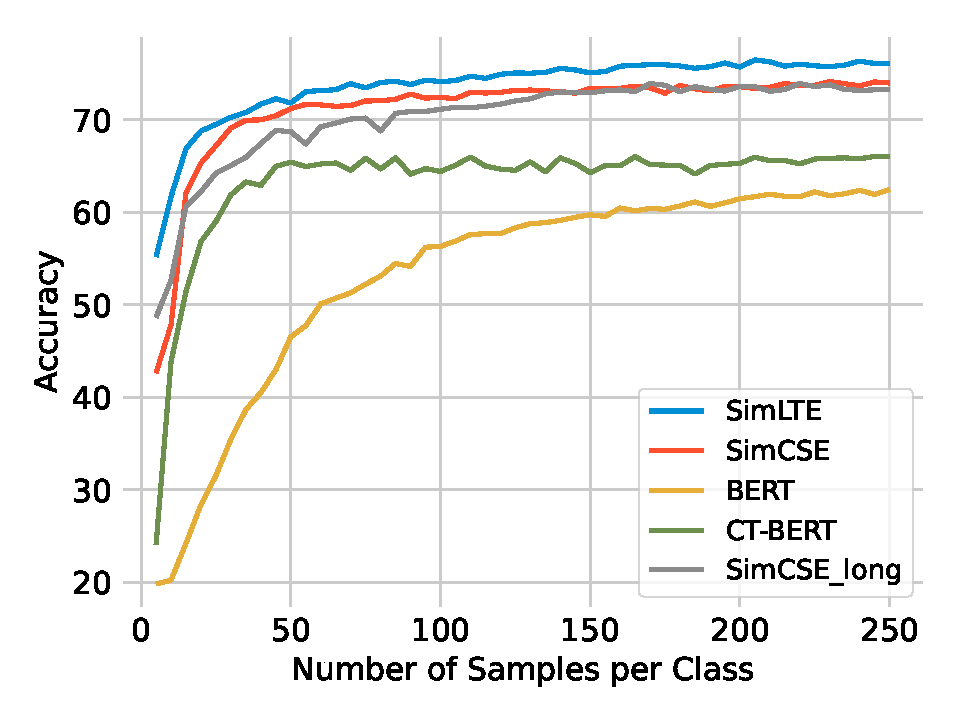
\includegraphics[width=0.8\linewidth]{fig/few_shot.pdf}
\caption{Performance of different models with different numbers of instances per class under few-shot setting.}
\label{few_shot}
\end{figure}

\textbf{Results.} 
Table~\ref{results} shows the results of few-shot text classification on these five datasets. 
We can see that \our~(i.e.,~\our$_{\mathrm{bert}}$ and \our$_{\mathrm{long}}$) achieves $12.0\%$ and $24.3\%$ macro-F1 improvements compared to SimCSE and Longformer respectively. These improvements are higher than general text classification. 
Besides, we also compare the performance of different baselines and \our$_{\mathrm{bert}}$ with different numbers of training instances on 20News. 
The results in Figure~\ref{few_shot} show the improvements from our method become larger as the number of training instances decreases indicating the importance of high-quality long text embeddings for low-resource settings. 
Furthermore, our method achieves the best results under different numbers of training instances.

\subsection{Attention Weights}
To explore the difference between \our~and other models, we analyze the attention weights of Transformers in different models on the NYT dataset (details in Appendix~\ref{app:attention}). The average weights of different kinds of words are shown in Figure~\ref{attentions}.  We can see that our model has more than $40\%$ higher attention weights on nouns compared to BERT and SimCSE. \citet{martin-johnson-2015-efficient} shows nouns are more informative than other words in the document understanding. Hence, our pretraining method increases the attention weights of models on nouns which results in higher performance on long text classification. 

\begin{figure}
\centering
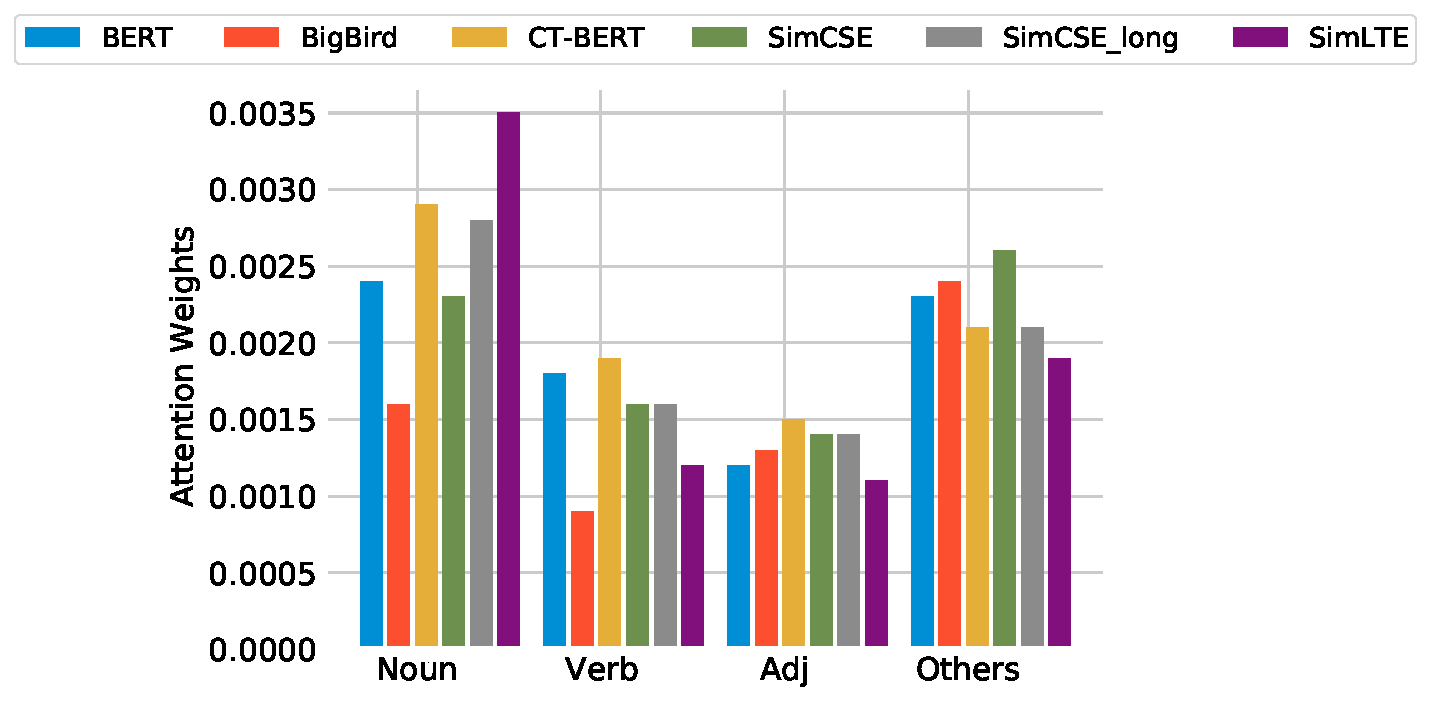
\includegraphics[width=0.8\linewidth]{fig/attentions.pdf}
\caption{Attention weights from different models on the NYT dataset.}  
\label{attentions}
\end{figure}

\section{Conclusion}
In this work, we propose an unsupervised contrastive learning framework for long text embeddings. 
Our method provides a new method for long text data augmentation without any supervision and language models can get large-scale pretraining on any long text. 
We conduct extensive experiments on text classification tasks under fully supervised and few-shot settings.
Results show that our pre-trained model greatly outperforms state-of-the-art text embeddings, especially when the training data is limited.

% Entries for the entire Anthology, followed by custom entries
\bibliography{anthology,custom}
\bibliographystyle{acl_natbib}

\clearpage
\appendix
\section{Redundancy}
\label{app:redundacy}
\begin{table}[h]
    \small
\begin{tabular}{l|cccccc}
\toprule
Length   & (1) & (2) & (3)   &  (4) &  (5)  & All\\
\midrule
FakeNews &1.06 &1.21 &29 &1.35 &1.52 &1.37 \\
20News &1.12 &1.18 &1.24 &1.31 &1.50 &1.28 \\
arXiv &1.12 &1.25 &1.36 &1.49 &1.62 &1.34\\
NYT &1.00 &1.14 &1.21 &1.31 &1.48 &1.45\\
BBCNews &1.05 &1.14 &1.20 &1.29 &1.46 &1.19 \\
\bottomrule
\end{tabular}
    \caption{Information redundancies for different lengths (i.e.,~word numbers) of text: (1) 0-50 (2) 51-100 (3) 101-200 (4) 201-300 (5) more than 300.}
    \label{redundancy}
\end{table}

We evaluate the redundancy of the text by counting the repeated verbs and nouns in the text. Specifically, we first use SpaCy~\footnote{https://spacy.io/} to find verbs and nouns and get their lemmatizations. Intuitively, if the redundancy of a document is high, nouns and verbs will be repeated frequently to express the same topic. Hence, redundancies $R$ in our paper are computed as:
\begin{equation}
    R = \frac{N_{\mathrm{nouns, verbs}}}{D_{\mathrm{nouns, verbs}}}
\end{equation}
where $N_{\mathrm{nouns, verbs}}$ denotes the number of nouns and verbs in a document and $D_{\mathrm{nouns, verbs}}$ is the number of distinct nouns and verbs.


\section{Training Details}
\label{app:details}
For text classification, the learning rate for fine-tuning is 3e-4; the batch size is 8; the maximum sequence length is 512 tokens. 
We fine-tune the last MLP layer on these five datasets and evaluate the classification performance with accuracy and macro-F1 scores.
For few-shot text classification, we sample 10 data instances per class for the FakeNewsCorpus dataset and the arXiv dataset and 5 data instances per class for the other three datasets. 
Other settings are the same as the general text classification. 
Since there is randomness in sampling, we repeat every experiment 10 times and take the average value of metrics.

\section{Attention Weights}
\label{app:attention}
We compute the attention weights for Transformers as follows:
(1) we first extract the attention weights between \texttt{[CLS]} token and all the other tokens;
(2) we compute the averaged weights along different heads in multi-head attention;
(3) the attention weights of the last layer in Transformers are used as the weights for words.
Averaged values are computed for nouns, verbs, adjectives, and other words.

\end{document}
